\chapter{方案设计}
\label{cha:example}

\setmonofont{Cascadia Code}
\newfontfamily\cyrillicfonttt{Cascadia Code}
\newfontfamily\englishfonttt{Cascadia Code}

\lstset{
    basicstyle = \small\ttfamily,
    tabsize=4
}

\section{课程作业目的}

\section{场景设计与预期要求}

\section{实现方案与技术细节}

\subsection{传统路由和基于TCP与UDP路由的实现方案}

\subsection{实现传统路由}

\subsubsection{搭建拓扑}

首先找到 \texttt{classic/create\_{}topo.py} 这个文件,
在配置好mininet的主机$A$中运行
\begin{lstlisting}
	sudo mn --custom create_topo.py --topo mytopo \
	--switch ovs --controller remote,ip={ip of B} --link tc
\end{lstlisting}

其中 \texttt{ip} 项是控制器主机$B$的 ip 地址。

在$B$主机中运行

\begin{lstlisting}
	ryu run --observe-links  \
	ryu.app.rest_router ryu.app.gui_topology.gui_topology
\end{lstlisting}

这样一来整个拓扑已经搭建成功。浏览 \texttt{http://ip\_of\_B:8080} 可以查看拓扑图像如下:

\begin{figure}[h]
	\centering
	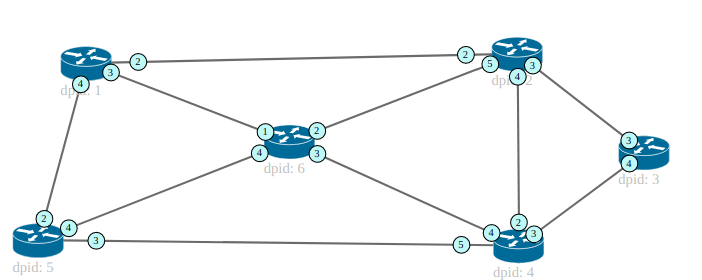
\includegraphics[width=0.5\textwidth]{image/topo1.png}
	\caption{拓扑图}
 	\label{fig:hole}
\end{figure}


注意到这里没有画出主机的拓扑情况。

\subsubsection{生成路由}

首先找到 \texttt{classic/make\_route.py},在主机$B$上运行

\begin{lstlisting}
	python make_route.py
\end{lstlisting}

这会在控制器上创建基于最短路算法的静态路由。
此时路由已经创建好,但是,由于主机的默认网关均未进行配置,要手动配置默认网关。

在mininet的命令行中运行

\begin{lstlisting}
	u1 ip route add default via 172.18.0.2 \
	u2 ip route add default via 172.18.1.2 \
	u3 ip route add default via 172.18.2.2 \
	u4 ip route add default via 172.18.3.2 \
	u5 ip route add default via 172.18.4.2 \
	u6 ip route add default via 172.18.2.2 \
	u7 ip route add default via 172.18.2.2 \
	u8 ip route add default via 172.18.2.2
\end{lstlisting}

这样一来路由就搭建成功了。

\subsubsection{测试路由}

在mininet的命令行中运行

\begin{lstlisting}
	pingall
\end{lstlisting}

得到输出如下:

\begin{lstlisting}
	mininet> pingall
	*** Ping: testing ping reachability
	u1 -> u2 u3 u4 u5 u6 u7 u8 
	u2 -> u1 u3 u4 u5 u6 u7 u8 
	u3 -> u1 u2 u4 u5 u6 u7 u8 
	u4 -> u1 u2 u3 u5 u6 u7 u8 
	u5 -> u1 u2 u3 u4 u6 u7 u8 
	u6 -> u1 u2 u3 u4 u5 u7 u8 
	u7 -> u1 u2 u3 u4 u5 u6 u8 
	u8 -> u1 u2 u3 u4 u5 u6 u7 
	*** Results: 0% dropped (56/56 received)
\end{lstlisting}

这样一来就可以确定路由已经正常工作。

\subsubsection{性能测试}

在mininet的命令行中运行

\begin{lstlisting}
	u3 iperf3 -s -D
	u6 iperf3 -s -D
	u7 iperf3 -s -D
	u8 iperf3 -s -D
	u1 iperf3 -c u3 -t 20 > u1.tcp &
	u1 iperf3 -c u6 -u -b 40M > u1.udp &
	u2 iperf3 -c u7 -t 20 > u2.tcp &
	u2 iperf3 -c u8 -u -b 40M > u2.udp &
\end{lstlisting}

性能测试的结果在 \texttt{u1.tcp, u1.udp, u2.tcp, u2.udp} 这四个文件中。

\subsection{实现基于UDP和TCP选择的SDN路由}

\subsubsection{搭建拓扑}

首先找到 \texttt{classic/create\_{}topo.py} 这个文件,
在配置好mininet的主机$A$中运行
\begin{lstlisting}
	sudo mn --custom create_topo.py --topo mytopo \
	--switch ovs --controller remote,ip={ip of B} --link tc
\end{lstlisting}

其中 \texttt{ip} 项是控制器主机$B$的 ip 地址。

在$B$主机中运行

\begin{lstlisting}
	ryu run --observe-links  \
	ryu.app.rest_router ryu.app.gui_topology.gui_topology \
	ryu.app.ofctl_rest
\end{lstlisting}

这样一来整个拓扑已经搭建成功。实际上,这里的拓扑和传统路由时的拓扑没有区别。

\subsubsection{生成路由}
首先找到 \texttt{sdn-tcp-udp} 文件夹中的 
\texttt{make\_classic\_route.py}和
\texttt{make\_sdn\_route.py},
在主机$B$上运行

\begin{lstlisting}
	python make_classic_route.py \
	python make_sdn_route.py
\end{lstlisting}

这会在控制器上创建基于最短路算法的静态路由和基于UDP和TCP的SDN路由。

此时路由已经创建好,但是,由于主机的默认网关均未进行配置,要手动配置默认网关。

在mininet的命令行中运行

\begin{lstlisting}
	u1 ip route add default via 172.18.0.2 
	u2 ip route add default via 172.18.1.2
	u3 ip route add default via 172.18.2.2
	u4 ip route add default via 172.18.3.2
	u5 ip route add default via 172.18.4.2
	u6 ip route add default via 172.18.2.2
	u7 ip route add default via 172.18.2.2
	u8 ip route add default via 172.18.2.2
\end{lstlisting}

这样一来路由就搭建成功了。

\subsubsection{测试路由}

在mininet的命令行中运行

\begin{lstlisting}
	pingall
\end{lstlisting}

得到输出如下:

\begin{lstlisting}
	mininet> pingall
	*** Ping: testing ping reachability
	u1 -> u2 u3 u4 u5 u6 u7 u8 
	u2 -> u1 u3 u4 u5 u6 u7 u8 
	u3 -> u1 u2 u4 u5 u6 u7 u8 
	u4 -> u1 u2 u3 u5 u6 u7 u8 
	u5 -> u1 u2 u3 u4 u6 u7 u8 
	u6 -> u1 u2 u3 u4 u5 u7 u8 
	u7 -> u1 u2 u3 u4 u5 u6 u8 
	u8 -> u1 u2 u3 u4 u5 u6 u7 
	*** Results: 0% dropped (56/56 received)
\end{lstlisting}

这样一来就可以确定路由已经正常工作。

\subsubsection{性能测试}

这里进行了两次性能测试,一次测试和传统路由相同,限制udp的速率为$40 Mbp/s$,
一次把udp的速率限制到$100 Mbp/s$。

在mininet的命令行中运行

\begin{lstlisting}
	u3 iperf3 -s -D
	u6 iperf3 -s -D
	u7 iperf3 -s -D
	u8 iperf3 -s -D

	u1 iperf3 -c u3 -w 1M -t 20 > u1-40.tcp &
	u1 iperf3 -c u6 -u -b 40M > u1-40.udp &
	u5 iperf3 -c u7 -w 1M -t 20 > u5-40.tcp &
	u5 iperf3 -c u8 -u -b 40M > u5-40.udp &

	u1 iperf3 -c u3 -w 1M -t 20 > u1-100.tcp &
	u1 iperf3 -c u6 -u -b 100M > u1-100.udp &
	u5 iperf3 -c u7 -w 1M -t 20 > u5-100.tcp &
	u5 iperf3 -c u8 -u -b 100M > u5-100.udp &
\end{lstlisting}

第一次性能测试的结果在 \texttt{u1-40.tcp, u1-40.udp, u5-40.tcp, u5-40.udp} 这四个文件中。

第二次性能测试的结果在 \texttt{u1-100.tcp, u1-100.udp, u5-100.tcp, u5-100.udp} 这四个文件中。

\section{组员的分工与工作}

1\cite{long2015fully}

\section{实验中遇到的挑战与问题及其解决方法}